\section{Улучшенная оценка смещения}

Оказывается, что существует лучший метод, чем \ref{eq10.4}, для аппроксимации $\widehat{\text{bias}}_{\infty} = \text{bias}_{\hat{F}}$ из $B$ бутстреп репликаций. Улучшенный метод применяется, когда $\hat{\theta}$ --- это плагин оценка $t(\hat{F})$ для $\theta = t(F)$. Мы описываем метод здесь и даем объяснение, почему он работает, в главе 23.

Нам нужно определить понятие вектора повторной выборки (???resampling vector). Пусть $P_{j}^{*}$ указывает долю бутстреп наблюдений $x^{*} = (x_{1}^{*}, x_{2}^{*}, \dots, x_{n}^{*})$, которая равна $j$-ому исходному наблюдению,
\begin{equation}
    P_{j}^{*} = \#\{x_{j}^{*} = x_{j}\}/n,\quad\quad j = 1, 2, \dots, n.
\end{equation}
Вектор повторной выборки
\begin{equation}\label{eq10.18}
    P^{*} = (P_{1}^{*}, P_{2}^{*}, \dots, P_{n}^{*})
\end{equation}
имеет неотрицательные компоненты в сумме дающие единицу. Например, третья бутстреп выборка для данных пластыря была $$X^{*} = (x_1, x_6,x_6, x_5, x_7, x_1, x_3, x_8)$$ и соответствующий вектор повторной выборки $$P^* = (2/8, 0, 1/8, 0, 1/8,2/8, 1/8, 1/8).$$

Бутстреп репликацию $\hat{\theta}^{*} = s(x^{*})$ можно рассматривать как функцию вектора повторной выборки $P^{*}$. Например, если $\hat{\theta} = \Bar{y}/\Bar{z}$ в \ref{eq10.10},
\begin{equation}\label{eq10.19}
   \hat{\theta}^{*} = \Bar{y}^{*}/\Bar{z}^{*} = \frac{\sum_{i=1}^{8}P^{*}_{j}y_{i}/8}{\sum_{i=1}^{8}P^{*}_{j}z_{i}/8}.
\end{equation}
(Обратите внимание, что исходные данные $x$ считаются фиксированными в этом определении; единственными случайными величинами являются $P_{j}^{*}$.) Для $\hat{\theta} = t(\hat{F})$, плагин оценки $\theta$, запишем
\begin{equation}\label{eq10.20}
   \hat{\theta}^{*} = T(P^{*})
\end{equation}
чтобы определить $\hat{\theta}^{*}$ как функцию вектора повторной выборки. \footnote{Мы обозначаем плагин статистику двумя способами $\hat{\theta} = s(x) = t(\hat{F})$. Аналогично бутстреп репликации обозначаются $\hat{\theta}^{*} = s(x^{*}) = T(P^{*})$. Три функции $s(\cdot)$, $t(\cdot)$ и $T(\cdot)$ представляют одну и ту же статистику, но рассматриваются как функция в трех разных пространствах.} Формула \ref{eq10.19} определяет $T(\cdot)$ для $\hat{\theta} = \Bar{y}/\Bar{z}$. 

Пусть $P^{0}$ обозначает вектор длины $n$, все элементы которого равны $1/n$,
\begin{equation}\label{eq10.21}
   P^{0} = (1/n, 1/n, \dots, 1/n).
\end{equation}
Значение $T(P^{0})$ --- это значение $\hat{\theta}^{*}$, когда каждый элемент $P_{j}^{*} = 1/n$, то есть когда каждая точка исходных данных $x_j$ встречается ровно один раз в бутстреп выборке $x^{*}$. Это означает, что $x^{*} = x$, за исключением, возможно, перестановок порядка, в котором появляются элементы $x_{1}, x_{2}, \dots, x_{n}$. Но статистика вида $\hat{\theta} = t(\hat{F})$ не меняется, когда элементы $x = (x_1, x_2, \dots, x_n)$ переупорядочиваются, потому что $F$ не изменяется. Другими словами,
\begin{equation}\label{eq10.22}
   T(P^{0}) = \hat{\theta} = t(\hat{F}),
\end{equation}
наблюдаемое выборочное значение статистики. (Это легко проверить в \ref{eq10.19}.)

$B$ бутстреп выборок $x^{*1}, x^{*2}, \dots, x^{*B}$ приводят к соответствующим векторам повторной выборки $P^{*1}, P^{*2}, \dots, P^{*B}$, каждый вектор $P^{*b}$ имеет форму \ref{eq10.18}. Определим $\Bar{P}^{*}$ как среднее значение этих векторов
\begin{equation}\label{eq10.23}
   \Bar{P}^{*} = \sum\limits_{i=1}^{B}P^{*b}/B.
\end{equation}
Согласно \ref{eq10.22} мы можем записать бутстреп оценку смещения \ref{eq10.4} в виде
\begin{equation}\label{eq10.24}
   \widehat{\text{bias}}_{B} = \hat{\theta}^{*}(\cdot) - T(P^{0}).
\end{equation}
Улучшенная бутстреп оценка смещения, которую мы обозначим как $\overline{\text{bias}}_{B}$, равна
\begin{equation}\label{eq10.25}
   \overline{\text{bias}}_{B} = \hat{\theta}^{*}(\cdot) - T(\bar{P}^{0}).
\end{equation}
Для рисунка 10.1 четыреста векторов повторной выборки усреднены до  $\bar{P}^{*}~=~(0.1178, 0.1187, 0.1313, 0.1259, 0.1219, 0.1275, 0.1306, 0.1213)$. Это приводит к
\begin{equation}\label{eq10.26}
  T(\bar{P}^{*}) = \frac{\sum_{i=1}^{8}\bar{P}^{*}_{j}y_{i}}{\sum_{i=1}^{8}\bar{P}^{*}_{j}z_{i}} = -0.0750
\end{equation}
и
\begin{equation}\label{eq10.27}
  \overline{\text{bias}}_{400} = -0.0670 - (-0.0750) = 0.0080,
\end{equation}
в отличие от $\widehat{\text{bias}}_{400} = 0.0043$.

Обе оценки $\widehat{\text{bias}}_{B}$ и $\overline{\text{bias}}_{B}$ сходятся к $\widehat{\text{bias}}_{\infty} = \text{bias}_{\hat{F}}$, идеальной бутстреп оценке смещения, когда $B$ стремится к бесконечности. Для $\overline{\text{bias}}_{B}$ сходимость происходит намного быстрее, поэтому мы назвали её улучшенной. Более быстрая сходимость очевидна на рисунке 10.2, на котором рассмотрены $\widehat{\text{bias}}_{B}$ и $\overline{\text{bias}}_{B}$ для $B$, равного $25, 50, 100, 200, 400, 800, 1670, 3200$. Предельное значение $\widehat{\text{bias}}_{\infty}$ было аппроксимировано $\widehat{\text{bias}}_{100000}= 0.0079$, показанным пунктирной горизонтальной линией. $\overline{\text{bias}}_{B}$ плавно и быстро приближается к пунктирной линии, в то время как $\widehat{\text{bias}}_{B}$ все еще довольно изменчива даже для $B = 3200$.

В главе 23 обсуждаются улучшенные вычислительные бутстреп методы. Там будет показано, что $\overline{\text{bias}}_{B}$ сводится к использованию $\widehat{\text{bias}}_{CB}$, где $C$ --- большая константа, часто $50$ или больше. Задача 10.7 предлагает одну причину превосходства $\overline{\text{bias}}_{B}$.

\noindent
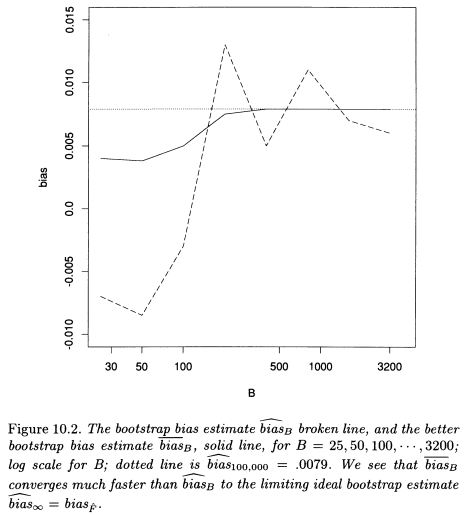
\includegraphics[width=\linewidth]{10/f10.2.png}
\newline